\section{Five-observable cross section}
\label{sec:part-illustrative-multidimensional}

We report the \resSixteen{} as cell integrals in $(p_T,p_\parallel,E_{\mathrm{avail}},q_3,W)$ for descriptive comparisons with generator predictions. The five reconstructed observables use four detector quantities (Sec.~\ref{sec:observable-definitions}). The muon-quadrant sums pass the prespecified agreement rule against the 2D result (Sec.~\ref{sec:sixteen-cell-projections}). The calibrated \resJoint{} reject every specified hybrid hypothesis. A post hoc check finds each rejection also visible in a matched coarse projection (Sec.~\ref{sec:sixteen-cell-generator-comparison}).

\subsection{Sixteen-cell cross section and uncertainty budget}
\label{sec:sixteen-cell-results}
\label{sec:fived16}
\label{sec:fived16-result}

Table~\ref{tab:sixteen-cell-cross-sections} and Fig.~\ref{fig:fived16-headline} give the flux-averaged cross section per nucleon integrated over each region in $(p_T,p_\parallel,E_{\mathrm{avail}},q_3,W)$. The integrals span $\fvval{f-R07}$ to $\fvval{f-R14}$ in units of $\fvval{f-unit}\,\mathrm{cm}^2$ per nucleon and sum to $\fpeval{round((\fvval{cr-QA-s16}+\fvval{cr-QB-s16}+\fvval{cr-QC-s16}+\fvval{cr-QD-s16})/10,3)}\times10^{-38}\,\mathrm{cm}^2$ per nucleon over the reported regions. In both low-$p_T$ quadrants, the largest contributions come from the low-$E_{\mathrm{avail}}$, low-$q_3$ cell and the high-$q_3$, high-$W$ cell. The high-$q_3$, high-$W$ cell in the high-$p_T$, high-$p_\parallel$ quadrant (R14) contributes the most overall.

\begin{figure}[!hbp]
  \centering
  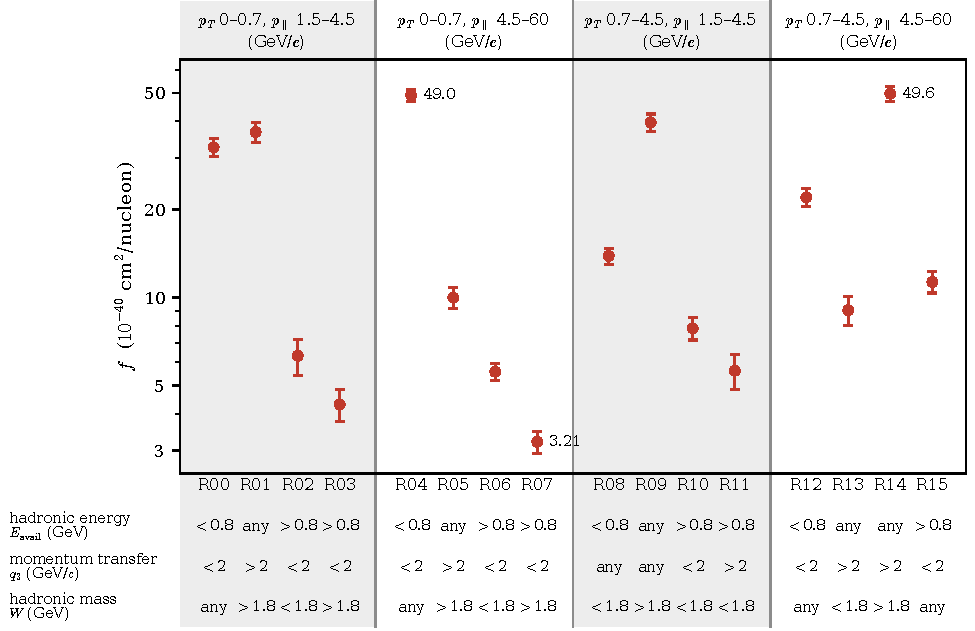
\includegraphics[width=\linewidth]{figures/fived16_headline.pdf}
  \caption{The sixteen cell integrals of the \resSixteen{} range from $\fvval{f-R07}$ (R07) to $\fvval{f-R14}$ (R14) in units of $\fvval{f-unit}\,\mathrm{cm}^2$ per nucleon. The covariance includes no term estimated from closure at held-out tunes and is too small for the deviations from truth there. See Secs.~\ref{sec:closure-interval-diagnostics} and~\ref{sec:result-validity} for the limits on using these uncertainties. The points are grouped by muon quadrant, with alternate quadrants shaded. The bars show standard deviations $\sqrt{(C_{\mathrm{rep}})_{ii}}$ on a logarithmic cross-section axis. The three rows below the axis give each cell's range in hadronic energy $E_{\mathrm{avail}}$, momentum transfer $q_3$ and hadronic mass $W$, with \emph{any} denoting the full interval in Table~\ref{tab:five-dimensional-regions}.}
  \label{fig:fived16-headline}
\end{figure}

\begin{table}[htbp]
  \centering\footnotesize
  \caption{Cell-integrated cross sections $f_i$ in units of $\fvval{f-unit}\,\mathrm{cm}^2$ per nucleon and total fractional standard deviations $100\sqrt{(C_{\mathrm{rep}})_{ii}}/f_i$. The cell definitions are given in Table~\ref{tab:five-dimensional-regions}.}
  \label{tab:sixteen-cell-cross-sections}
  \label{tab:fived16-cells}
  \begin{tabular}{@{}lrr@{}}
    \toprule
    Cell & $f_i$ & Total (\%) \\
    \midrule
    R00 & \fvval{f-R00} & \fvval{sig-reported-R00} \\
    R01 & \fvval{f-R01} & \fvval{sig-reported-R01} \\
    R02 & \fvval{f-R02} & \fvval{sig-reported-R02} \\
    R03 & \fvval{f-R03} & \fvval{sig-reported-R03} \\
    \addlinespace[2pt]
    R04 & \fvval{f-R04} & \fvval{sig-reported-R04} \\
    R05 & \fvval{f-R05} & \fvval{sig-reported-R05} \\
    R06 & \fvval{f-R06} & \fvval{sig-reported-R06} \\
    R07 & \fvval{f-R07} & \fvval{sig-reported-R07} \\
    \addlinespace[2pt]
    R08 & \fvval{f-R08} & \fvval{sig-reported-R08} \\
    R09 & \fvval{f-R09} & \fvval{sig-reported-R09} \\
    R10 & \fvval{f-R10} & \fvval{sig-reported-R10} \\
    R11 & \fvval{f-R11} & \fvval{sig-reported-R11} \\
    \addlinespace[2pt]
    R12 & \fvval{f-R12} & \fvval{sig-reported-R12} \\
    R13 & \fvval{f-R13} & \fvval{sig-reported-R13} \\
    R14 & \fvval{f-R14} & \fvval{sig-reported-R14} \\
    R15 & \fvval{f-R15} & \fvval{sig-reported-R15} \\
    \bottomrule
  \end{tabular}
\end{table}

\phantomsection
\label{sec:fived16-cov}
The reported covariance in Eq.~\eqref{eq:sixteen-cell-covariance} gives a median per-cell uncertainty of $\fvval{sigmed-reported}\%$. Flux and prior-shape variations give the largest median contributions. Lateral variations and the spread across run periods also contribute appreciably. Prior-shape sensitivity gives fractional standard deviations above $\fpeval{floor(min(\fvval{sig-C_model-R02},\fvval{sig-C_model-R03},\fvval{sig-C_model-R11}))}\%$ in R02, R03, and R11. The energy-response term increases the standard deviation relative to the subtotal before response and run-period terms by up to $\fpeval{round(100*(\fvval{sigratio-max}-1),0)}\%$ in one cell. The reported covariance includes prior-shape sensitivity. It has no term estimated from closure at held-out tunes. It also remains too small for the deviations from truth when used to rescore the held-out pseudo-experiments (Sec.~\ref{sec:sixteen-cell-closure-tunes}). Appendix~\ref{app:higher-dimensional-projections} gives the cell-by-cell decomposition and the correlation matrix.

\subsection{Projection consistency and run-period differences}
\label{sec:sixteen-cell-projections}
\label{sec:fived16-quadrants}

Summing the sixteen-cell result over the hadronic coordinates gives four coarse muon integrals within $\fpeval{round(abs(\fvval{cr-QC-dpct}),1)}\%$ of the 2D OmniFold result. Table~\ref{tab:five-dimensional-regions} orders the quadrants defined by $p_T=\fvval{h2-mid-pt}~\mathrm{GeV}/c$ and $p_\parallel=\fvval{h2-mid-pz}~\mathrm{GeV}/c$. In that order the differences from 2D are $+\fpeval{round(\fvval{cr-QA-dpct},2)}\%$, $\fpeval{round(\fvval{cr-QB-dpct},2)}\%$, $\fpeval{round(\fvval{cr-QC-dpct},2)}\%$, and $+\fpeval{round(\fvval{cr-QD-dpct},2)}\%$. The largest fractional difference is in the high-$p_T$, low-$p_\parallel$ quadrant. The sum over all four quadrants is $\fpeval{round(100*(1-(\fvval{cr-QA-s16}+\fvval{cr-QB-s16}+\fvval{cr-QC-s16}+\fvval{cr-QD-s16})/(\fvval{cr-QA-s2}+\fvval{cr-QB-s2}+\fvval{cr-QC-s2}+\fvval{cr-QD-s2})),2)}\%$ below the 2D integral.

All four differences pass the prespecified agreement rule. Appendix~\ref{app:higher-dimensional-projections} gives the assumed-correlation thresholds and the scan over constructed cross-covariances.

The sixteen-cell quadrant sums are $\fvval{g3d-pct-lo}\%$ to $\fvval{g3d-pct-hi}\%$ below the corresponding 3D central values. The largest difference is $\fvval{g3d-zmax}$ times the reported sixteen-cell standard deviation of the relevant sum. Because the 3D result has no reported covariance, this comparison cannot quantify their statistical agreement. Changes that redistribute cross section between hadronic cells within a muon quadrant cancel in these sums.

\phantomsection
\label{sec:fived16-pl}
The data from different run periods show a longitudinal-momentum step before any unfolding (Fig.~\ref{fig:runperiod-steps}). Across $p_\parallel=8~\mathrm{GeV}/c$, the reconstructed double ratio steps by $+\fvval{rp-pb-reco}\%$ for the middle group and $+\fvval{rp-pc-reco}\%$ for the latest group, each relative to the earliest group. In separate five-observable unfoldings, the middle-to-earliest double ratio of unfolded to simulated cross sections has a step of $(\fvval{rpd-s0}\pm\fvval{rpd-s0-sigma})\%$, where the uncertainty is the bootstrap scatter. The three groups' unfolded data-to-simulation ratios also differ on the sixteen cells by more than the variation among bootstrap replicas. The cause of the inconsistency is unidentified, and these data cannot establish which period, if any, is right.

\begin{figure}[!hbp]
  \centering
  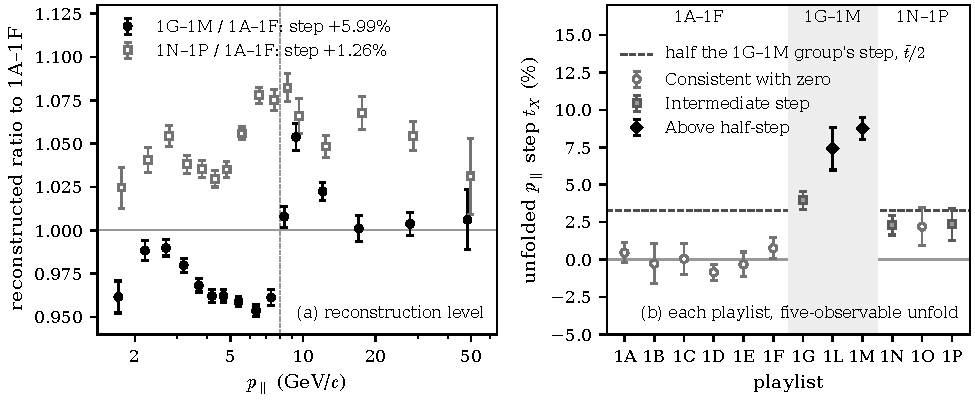
\includegraphics[width=\linewidth]{figures/runperiod_steps.pdf}
  \caption{A step across $p_\parallel=8~\mathrm{GeV}/c$ is already visible before unfolding. Run groups are early (1A--1F), middle (1G--1M), and late (1N--1P). Panel (a) divides the reconstructed ratio of background-subtracted data to exposure-scaled signal simulation in each $p_\parallel$ bin, summed over $p_T$, by the same ratio for the early group. Bars show data statistical uncertainties. Panel (b) shows the five-observable unfolded step for each individual run period relative to the early group, leaving that period out of the reference if it belongs to the group. Bars show bootstrap standard deviations. Open circles mark steps consistent with zero within two standard deviations. Filled diamonds mark steps that exceed half the middle group's step (dashed line, recombined from its three periods) by two standard deviations of the difference. Squares mark the remaining steps. The symbols establish neither the location nor the cause of the step.}
  \label{fig:runperiod-steps}
\end{figure}

The run-period covariance represents the spread of the three groups across the sixteen integrals. It was constructed after the differences were observed, and its scale and coverage have had no independent validation. Appendix~\ref{app:covariance-construction} gives the construction and rank, and Appendix~\ref{app:choices-after-results} records the timing.
% Search: run-period covariance validation; run-period block scale; C_PL coverage; C_run coverage test; RPD; RPD-RECO; REGRADE (DECISION-20261102-joseph-quadrant-sentence-sec4-and-validations.md:30: the block's size cannot be validated with three groups; RPD and RPD-RECO diagnose its cause; REGRADE grades toys against C_rep, which includes the block, and does not validate its scale) @ caae27166e85

\subsection{Comparison with generator predictions}
\label{sec:sixteen-cell-generator-comparison}
\label{sec:fived16-gen}

All three hydrocarbon predictions lie below the unfolded integrals in every high-$p_T$ cell. Figure~\ref{fig:sixteen-cell-generator-residuals} compares the sixteen integrals with GENIE 2.12.10~\cite{Andreopoulos:2009rq} without and with the Valencia meson-exchange current (MEC) contribution and with MINERvA Tune v1, the unfolding prior. We also compare with NuWro 21.09~\cite{Golan:2012wx} and GiBUU 2019~\cite{Buss:2011mx} on carbon. All predictions use the analysis definitions of $W$ and the muon angle. The generated GiBUU sample ends at $E_\nu=\fvval{cmodel-gibuu-enu}~\mathrm{GeV}$, so the sixteen-cell comparison with GiBUU uses the eight cells with $p_\parallel<\fvval{h2-mid-pz}~\mathrm{GeV}/c$, which contain about $\fpeval{round(100*(\fvval{cr-QA-s16}+\fvval{cr-QC-s16})/(\fvval{cr-QA-s16}+\fvval{cr-QB-s16}+\fvval{cr-QC-s16}+\fvval{cr-QD-s16}),0)}\%$ of the reported cross section. The data are normalized per nucleon of hydrocarbon (CH).

\begin{figure}[!hbp]
  \centering
  % Series targets and the GiBUU cell count verified against inputs2/fived16_genresidual_values.json.
  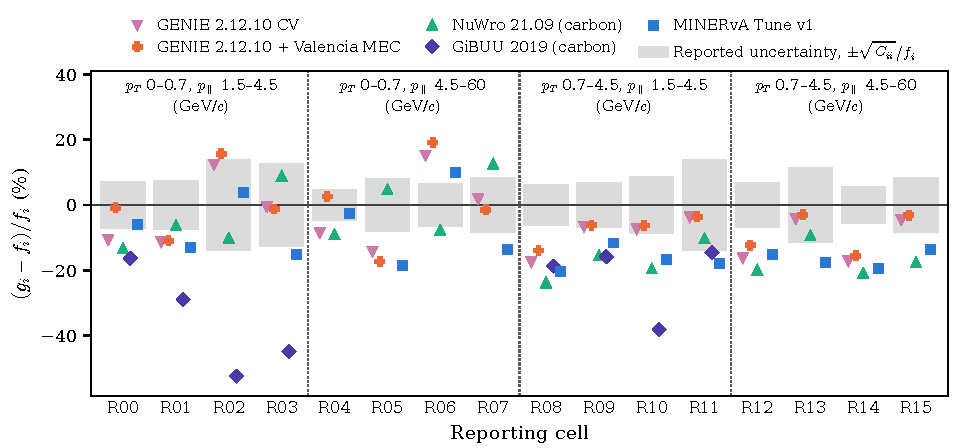
\includegraphics[width=\linewidth]{figures/fived16_genresidual.pdf}
  \caption{All three hydrocarbon predictions lie below the unfolded integrals in every high-$p_T$ cell. The points show the fractional differences $(g_i-f_i)/f_i$ between the predicted cell integrals $g_i$ and the unfolded cell integrals $f_i$ of the \resSixteen{}, on hydrocarbon for GENIE and Tune v1 and on carbon for NuWro and GiBUU (GiBUU on its eight cells). The gray bars show $\pm\sqrt{(C_{\mathrm{rep}})_{ii}}/f_i$ about zero using only the diagonal of $C_{\mathrm{rep}}$, with correlations and $V_g$, the diagonal covariance from finite generator statistics, entering the distances in Table~\ref{tab:sixteen-cell-model-distances}. Vertical separators indicate the four muon quadrants in Table~\ref{tab:five-dimensional-regions}. The points are offset horizontally within each cell to aid visibility.}
  \label{fig:sixteen-cell-generator-residuals}
\end{figure}

GENIE without Valencia MEC is below the unfolded result by $\fpeval{abs(\fvval{g-gcv-gf-R08})}\%$ in R08 and $\fpeval{abs(\fvval{g-gcv-gf-R14})}\%$ in R14. Both have $p_T\geq\fvval{h2-mid-pt}~\mathrm{GeV}/c$, but R08 selects low available energy and low hadronic mass, while R14 selects high momentum transfer and high hadronic mass. Adding Valencia MEC reduces these deficits to $\fpeval{abs(\fvval{g-gmec-gf-R08})}\%$ and $\fpeval{abs(\fvval{g-gmec-gf-R14})}\%$. It brings the prediction closer to the central value in R00, from $\fpeval{abs(\fvval{g-gcv-gf-R00})}\%$ below to $\fpeval{abs(\fvval{g-gmec-gf-R00})}\%$ below, at low $p_T$, $E_{\mathrm{avail}}$, and $q_3$. In both low-$p_T$ cells with high $E_{\mathrm{avail}}$, low $q_3$, and low $W$ (R02 and R06), GENIE already exceeds the central values by $\fpeval{round(\fvval{g-gcv-gf-R02},0)}$--$\fpeval{round(\fvval{g-gcv-gf-R06},0)}\%$ and the addition increases the excess to $\fpeval{round(\fvval{g-gmec-gf-R02},0)}$--$\fpeval{round(\fvval{g-gmec-gf-R06},0)}\%$. Tune v1 lies below the unfolded result in fourteen cells, with deficits of about $\fpeval{round((abs(\fvval{g-tune-gf-R08})+abs(\fvval{g-tune-gf-R14}))/2,0)}\%$ in R08 and R14.

Table~\ref{tab:sixteen-cell-model-distances} summarizes the differences using descriptive quadratic distances. For the rate-and-shape comparison the residual is $\boldsymbol{f}-\boldsymbol{g}$, with metric given by the inverse of $C_{\mathrm{rep}}+V_g$, where $V_g$ is the prediction's diagonal finite-sample covariance. The shape comparison uses unit-normalized cell fractions. Normalizing reduces the distance substantially for GiBUU on its eight-cell domain and more modestly for NuWro. For the two GENIE predictions and Tune v1, large distances persist after normalization. Of the predictions evaluated over all sixteen cells, the GENIE configuration without Valencia MEC has the smallest distance for both comparisons, even though the addition improves the agreement in several individual cells.

\begin{table}[htbp]
  \centering\footnotesize
  \caption{Descriptive quadratic distances for the generator comparisons. The target is carbon (C) or hydrocarbon (CH). The columns retain the rate and shape together ($\chi^2_{\mathrm{tot}}$) or the shape alone ($\chi^2_{\mathrm{sh}}$). The respective dimensions are \fvval{g-gcv-total-ndf} and \fvval{g-gcv-shape_only-ndf} for the full set of cells and \fvval{g-gibuu-total-ndf} and \fvval{g-gibuu-shape_only-ndf} for the GiBUU subset.}
  \label{tab:sixteen-cell-model-distances}
  \label{tab:fived16-gen}
  \begin{tabular}{@{}llrr@{}}
    \toprule
    Prediction & Target & Rate and shape & Shape only \\
    \midrule
    GENIE 2.12.10 & CH & \fvval{g-gcv-total-chi2} & \fvval{g-gcv-shape_only-chi2} \\
    GENIE + Valencia MEC & CH & \fvval{g-gmec-total-chi2} & \fvval{g-gmec-shape_only-chi2} \\
    NuWro 21.09 & C & \fvval{g-nuwro-carbon-total-chi2} & \fvval{g-nuwro-carbon-shape_only-chi2} \\
    \fvval{label-tune} & CH & \fvval{g-tune-total-chi2} & \fvval{g-tune-shape_only-chi2} \\
    GiBUU 2019 (8 cells) & C & \fvval{g-gibuu-carbon-total-chi2} & \fvval{g-gibuu-carbon-shape_only-chi2} \\
    \bottomrule
  \end{tabular}
\end{table}

The distances can change substantially with the covariance. Omitting the run-period term raises the rate-and-shape distance for NuWro from \fvval{g-nuwro-carbon-total-chi2int} to \fvval{g-nuwro-carbon-total-chi2int-nopl} (Appendix~\ref{app:higher-dimensional-projections}).

\phantomsection
\label{sec:joint5d}

The calibrated \resJoint{} reject all \jtNtests{} specified hybrid hypotheses at a familywise level of $\jtAlpha$. A hybrid hypothesis fixes the five-dimensional truth integrals in each fine cell to the generator prediction. It uses the Tune v1 event mixture within each fine cell, which the interaction-model bands vary during calibration while preserving the cell integral. The tests use a rate-and-shape and a shape-only hypothesis for each prediction and target in Table~\ref{tab:sixteen-cell-model-distances}. The statistic is a quadratic distance on \jtNcells{} supported cells of the separate coarse grid, or \jtNcellsGiBUU{} cells with $p_\parallel<6~\mathrm{GeV}/c$ for GiBUU. The shape statistic uses normalized cell fractions.

\phantomsection

\label{sec:joint5d-results}
\label{sec:joint5d-reading}
Pseudo-experiments calibrate each statistic by repeating the unfolding under its hybrid null with the specified nuisance variations (Appendix~\ref{app:joint-generator-tests}). The rejections concern these hybrid hypotheses and do not by themselves exclude a generator's nuclear model. The tests add no reportable uncertainty, and they neither use nor validate the covariance of the \resFiveAxis{}. The decisions hold under six conditions, listed in Appendix~\ref{sec:joint5d-conditions}. They include the calibration, for which no rejection rate has been measured for null pseudo-data processed like the data, and the detector response, whose specified variations include no dedicated calorimetric recoil-energy-scale variation.

In a post hoc check, every joint rejection also meets the single-test threshold $p<0.05$ in at least one matched coarse projection. The comparison repeats the calibration on $3\times3$ projections of the same joint cells onto $(p_T,p_\parallel)$ and $(E_{\mathrm{avail}},W)$. The finding holds both with the joint null shifts fixed and with shifts recomputed after projection. For GENIE without Valencia MEC, the projected $p$ values in the muon plane are \woneGcvPtTot{} for rate and shape and \woneGcvPtShape{} for shape alone. Both comparisons reject in the available-energy--hadronic-mass plane.

The projection criterion was set after the joint outcomes were known and before the projection comparison ran (Appendix~\ref{app:choices-after-results}). The five-observable tests show no evidence of discrimination beyond the matched coarse projections, and an independent test of the added discrimination remains open.
